\documentclass{standalone}
\usepackage{tikz}
\begin{document}
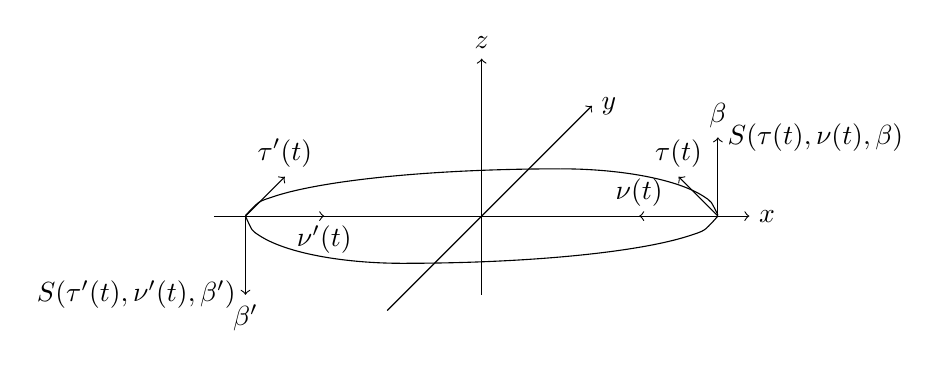
\begin{tikzpicture}[scale=2]
    \coordinate(O) at(0,0);
    \draw[->](-0.6,-0.6)--(0.7,0.7)node[right]{$y$};
    \draw[->](-1.7,0)--(1.7,0)node[right]{$x$};
    \draw[->](0,-0.5)--(0,1)node[above]{$z$};

    \draw[->](1.5,0)--(1,0)node[above]{$\nu(t)$};
    \draw[->](1.5,0)--(1.25,0.25)node[above]{${\tau}(t)$};
    \draw[->](1.5,0)--(1.5,0.5)node[above]{${\beta}$};
    \node[right]at(1.5,0.5){$S(\tau(t),\nu(t),\beta)$};


    \draw[->](-1.5,0)--(-1,0)node[below]{${\nu}'(t)$};
    \draw[->](-1.5,0)--(-1.25,0.25)node[above]{${\tau}'(t)$};
    \draw[->](-1.5,0)--(-1.5,-0.5)node[below]{${\beta}'$};
    \node[left]at(-1.5,-0.5){$S(\tau'(t),\nu'(t),\beta')$};

    \draw[-]plot[smooth, domain=-1.5:-0.5](\x,{-0.3*(1-(\x+0.5)^2)^0.5});
    \draw[-]plot[smooth, domain=0.5:1.5](\x,{0.3*(1-(\x-0.5)^2)^0.5});
    \draw[-]plot[smooth, domain=0.5:-1.5](\x,{0.15*(4-(\x-0.5)^2)^0.5});
    \draw[-]plot[smooth, domain=1.5:-0.5](\x,{-0.15*(4-(\x+0.5)^2)^0.5});
\end{tikzpicture}
\end{document}